\documentclass[sigconf,anonymous,review]{acmart}
\usepackage{booktabs}
\usepackage{amsmath}
\usepackage{amsthm}
\usepackage{tikz}
\usetikzlibrary{arrows.meta,positioning}
\newtheorem{theorem}{Theorem}
\newtheorem{proposition}{Proposition}
\newtheorem{definition}{Definition}
\newtheorem{lemma}{Lemma}
\bibliographystyle{ACM-Reference-Format}
\setlength{\emergencystretch}{1em}
\title{When Is an Agent Entitled to Claim Success?\\Verification Contracts for Open-World Outcomes}
\author{Anonymous Authors}
\keywords{AI agents, outcome verification, selective prediction, auditability}
\ccsdesc[500]{Computing methodologies~Intelligent agents}
\ccsdesc[300]{Software and its engineering~Software verification}
\begin{document}
\begin{abstract}
Agents increasingly perform tasks whose completion cannot be read from authoritative program state and is instead inferred from screenshots, images, documents, links, or bundles of contextual evidence. Existing systems often delegate this decision to a model judge. Yet even a confident and semantically correct judgment may not be eligible to trigger payment, access, completion, or workflow advancement: the acceptance rule may have changed after submission, evidence may belong to another task, unresolved uncertainty may have been forced into a binary answer, or the transition may be impossible to reconstruct.

We study a question distinct from improving judge accuracy: under what conditions may a probabilistic observation authorize a deterministic state transition? We first establish a \emph{separation} result---whenever a safe and an unsafe context are artifact-indistinguishable, an artifact-only judge cannot both authorize the safe member of that equivalence class and remain authorization-sound on the class---which places the problem outside the reach of better classification. We then introduce a \emph{Verification Contract}, a protocol that joins an outcome claim, ex-ante proof obligations, evidence binding, selective verification, admissible transitions, and a reconstructable receipt. We define four measurable properties---ex-ante consistency, evidence binding, selective safety, and decision reconstructability. Three of them (ex-ante consistency, evidence binding, reconstructability) are \emph{deterministic} checks over committed metadata and thus evaluate two-valuedly; the abstain value $?$ is needed only for the one \emph{probabilistic} predicate, selective verification, where a calibrated but uncertain observation must not be rounded into a forced binary. We give these predicates a common three-valued authorization semantics with a truth-biased guard and prove two \emph{interface} properties: a \emph{violation-propagation invariant}---a predicate value already known to be $\bot$ is never masked by satisfied or unresolved co-predicates (we deliberately avoid the word ``soundness'' so it is not misread as an empirical safety claim)---and \emph{abstention-monotonicity} (resolving an unknown never manufactures an unsafe permit). We are explicit that this invariant is conditional on a $\bot$ being correctly produced; it does not by itself certify that the underlying observation is correct, and it is therefore not an empirical safety advantage but a compositional invariant, whose real-world value the confirmatory study measures. The central \emph{theoretical} result is the capacity-independent \emph{context-collapse separation theorem}; the other two interface properties are auxiliary lemmas describing the guard's compositional behavior.

We design JOVE-Core, a grouped benchmark of consented digital base cases and property-aligned matched defects. Ground truth is an independently rated downstream harm---an erroneous payment, access grant, completion, or wrongful rejection of a legitimate submitter---judged by raters blind to the contract mechanism, so the metric does not reduce to the protocol's own rule. We preregister two separate endpoint groups: \emph{structural-consistency} endpoints ($P/B/R$, whose truth is fixed by deterministic recomputation against frozen commitments and which serve as an implementation-correctness check of the mechanism) and \emph{external-outcome} endpoints (the unsafe downstream harm, judged by blinded raters, which alone carry any empirical-superiority claim). The external-outcome primary comparison is paired at the preregistered matched automation coverage of 0.70; full risk--coverage curves and AURC are secondary analyses. Its primary contrast is the complete contract against an \emph{information-matched} judge that receives the identical evidence and observation payload but lacks structural enforcement; a strong policy-aware judge with an abstention interface and a deterministic tool-augmented judge are secondary references. This is a preregistered study manuscript following the Registered Report model: it fixes the problem, abstraction, per-field baseline construction, target sample size, statistical power, analysis scripts, and falsification criteria in advance. It makes no empirical superiority claim before confirmatory data are independently labeled and analyzed.
\end{abstract}
\maketitle

\section{Introduction}
Consider an agent that asks a user to publish a specified statement before a deadline. The user submits a plausible screenshot, and a multimodal judge reports success with 0.97 confidence. Should the system release payment? The question is no longer hypothetical: emerging agent-commerce and agent-payment protocols \cite{coinbase2025x402,google2025ap2,anthropic2024mcp,ethereum2025erc8004} let autonomous agents settle value over HTTP the moment an outcome is declared met, so a judge's belief is increasingly wired directly to an irreversible transfer.

The judgment is insufficient. The screenshot may be old, may belong to another campaign, or may have been produced under a different policy version. The requester may have changed the criterion after seeing the submission. A required provider may have failed while the application still demanded PASS or FAIL. The payment service may retain only a boolean and a transaction hash, leaving no way to recover which rule and evidence authorized the transfer.

These are not all classification errors. The judge may correctly recognize the screenshot's content while the transition remains impermissible. The missing object is the set of conditions under which a classification is allowed to control state.

Prior work addresses parts of this boundary. LLM-as-a-Judge studies evaluator agreement and bias \cite{zheng2023judging,liu2023geval,wang2024fair}. Selective prediction studies when a model should abstain \cite{geifman2017selective,geifman2019selectivenet,kamath2020selectiveqa,hendrickx2024reject}. Media forensics exposes artifact-level risk signals \cite{verdoliva2020media}. Agent benchmarks evaluate consequential workflows populated by increasingly autonomous, human-like agents \cite{liu2023agentbench,zhou2023webarena,xie2024osworld,xu2024theagentcompany,yang2024sweagent,park2023generative}, and a parallel safety literature documents \emph{why} their self-reported success cannot be trusted at face value: agents hallucinate outcomes \cite{ji2023hallucination}, act on injected or manipulated context \cite{greshake2023injection}, and take consequential but unsafe actions when sandboxed against realistic tools \cite{ruan2024toolemu,kang2024exploiting}. Human computation systems treat human labor as a programmable, quality-controlled resource for exactly the adjudication steps a machine cannot resolve \cite{kittur2011crowdforge,little2010turkit,retelny2014flashteams,franklin2011crowddb}, and acceptance criteria that shift over time are a recognized instance of concept drift \cite{gama2014survey}. Provenance and documentation practices record lineage and scope \cite{bender2018data,gebru2021datasheets,mitchell2019modelcards}. None alone determines when uncertain external evidence becomes eligible to authorize a downstream transition.

We call this the \emph{open-world outcome authorization} problem. It arises from an asymmetry: observations remain probabilistic, while consequences are discrete. A model can hold 0.73 belief; a payment system must release or withhold funds. Thresholding a score does not address policy drift, cross-task replay, provider failure, or irreconstructable decisions. In the blockchain setting this asymmetry is known as the \emph{oracle problem}---how off-chain, uncertain facts may legitimately authorize on-chain, deterministic, irreversible transfers \cite{caldarelli2020oracle,zhang2016towncrier,breidenbach2021chainlink}---and existing token standards \cite{vogelsteller2015erc20} standardize the transfer but not the evidential precondition for it. Even recent agent-facing on-chain standards that introduce identity, reputation, and validation registries \cite{ethereum2025erc8004} register \emph{party identity} and \emph{outcome records} rather than whether an \emph{uncertain} outcome is \emph{eligible}, under a frozen criterion and task binding, to authorize a transfer---the gap this paper fills. We treat open-world outcome authorization as the general form of this problem, independent of any ledger.

We introduce a \emph{Verification Contract}. It is neither a legal contract nor a formal proof of external truth. It is a machine-enforceable authorization boundary: obligations are committed before evidence; evidence is bound to task and version; unresolved states can halt automation; downstream actions are allowlisted; and each decision produces a reconstructable receipt.

Our contributions are:
\begin{enumerate}
\item We formulate open-world outcome authorization and prove a \emph{separation} (Theorem~\ref{thm:separation}): whenever a safe and an unsafe context share identical evidence, no artifact-only judge can both attain positive permit coverage on that ambiguous equivalence class and remain authorization-sound on it, so the deficiency is informational and interface-level rather than statistical.
\item We define Verification Contracts and a three-valued authorization semantics with a truth-biased guard, where the abstain value is exercised only by the probabilistic predicate and the other three predicates reduce to deterministic boolean checks. We prove three \emph{interface-level} properties of the guard and name them carefully so they are not overstated: a \emph{violation-propagation invariant} (Theorem~\ref{thm:soundness}: a value already known to be $\bot$ is never masked---we deliberately do not call this ``soundness''); \emph{abstention-monotonicity} (Proposition~\ref{prop:abstain}: resolving unknowns never creates an unsafe permit); and \emph{relative non-redundancy} (Theorem~\ref{thm:necessity}: relative to the enumerated defect family, dropping any one of the four properties reopens a matched harm the full guard blocks, with relative completeness over the modeled defect family in Proposition~\ref{prop:completeness}). These are compositional invariants over predicate values, not guarantees that a predicate observes external truth correctly; the empirical question of whether a $\bot$ is produced when it should be is deferred to the confirmatory study. The central \emph{theoretical} contribution of this paper is the capacity-independent separation result (Theorem~\ref{thm:separation}); violation-propagation and relative non-redundancy are auxiliary lemmas characterizing the guard's interface behavior and are not presented as empirical safety guarantees.
\item We design JOVE-Core so that each property corresponds to a controlled failure and an ablation, with ground truth anchored to independently rated downstream harm rather than to the contract's own rule.
\item We preregister an information-matched primary baseline, per-field baseline construction, risk--coverage evaluation, held-out generalization, human reconstruction, a target sample size with a power analysis, and explicit falsification conditions.
\end{enumerate}

We use ``open-world'' to name the observational regime---outcomes read from external evidence rather than authoritative program state---not a claim of coverage over physical, high-stakes, or adversarially unconstrained settings, which are outside the confirmatory scope. This is a preregistered study manuscript following the Registered Report model \cite{nosek2018preregistration,chambers2022registered}. Without confirmatory evidence, it cannot claim that Verification Contracts outperform policy-aware judging.

\section{Problem Formulation}
Let a requester or agent declare outcome $q$, an evidence producer submit $e$, a verifier obtain observations $o$, and a downstream application occupy state $s$. The application considers a positive consequential action $a^+$, such as releasing payment, granting access, marking completion, or crossing an irreversible workflow boundary.

A conventional judge implements
\begin{equation}
J(q,e)\rightarrow\{\mathrm{success},\mathrm{failure}\},
\end{equation}
possibly with confidence or rationale. This interface does not represent when the rule was fixed, to which task the artifact belongs, whether required services were available, how unknown propagates, which action is allowed, or how the decision can be reconstructed.

We define an \emph{unsafe positive transition} as execution of $a^+$ without satisfaction of the declared authorization conditions. This event is related to, but not identical with, a false-positive classification. A semantically correct observation can still be replayed from another task; a true outcome can still be judged under a policy invented after submission.

\subsection{Threat Model}
The producer may omit evidence, replay stale artifacts, substitute context, manipulate files, or exploit evaluator ambiguity. The requester may change criteria after submission. A provider may fail, drift, disagree, or emit malformed output. The application may map timeout, error, or abstention to success. An auditor may not receive private raw artifacts.

We do not assume honest metadata, independent model errors, perfect provenance, or unbiased human review. We do not cover every identity attack, sensor compromise, collusion strategy, or adaptive media attack.

\section{Why Judge Accuracy Is Insufficient}
We separate two kinds of counterexample. The first two bind directly to judge \emph{sufficiency}: even an oracle judge, given the artifact alone, lacks the information to authorize safely. The second two expose the \emph{deployment interface} around the judge; we state them as interface counterexamples, not as failures of classification, because a careful engineer could mitigate each without changing the judge.

\subsection{Counterexamples to judge sufficiency}
\paragraph{Post-hoc criterion drift.} After evidence arrives, the operative acceptance rule changes---for example, a view-count threshold is added. An oracle judge can apply either the old or the new rule correctly, yet no judgment can recover \emph{which} rule was in force when the evidence was produced. We distinguish this from a legitimate clarification: a requester refining a genuinely ambiguous criterion is benign, and the contract handles it by versioning obligations rather than by rewarding rejection. The defect is a silent change of the decisive rule against frozen evidence, not any post-submission communication.

\paragraph{Cross-task replay.} A screenshot correctly contains the required statement but belongs to another account, task, or policy version. Semantic correctness does not establish task membership; the judge, seeing only the artifact, cannot in principle distinguish a bound submission from a replayed one.

\subsection{Counterexamples to the deployment interface}
\paragraph{Forced binary output.} A required provider is unavailable or a mandatory modality is unsupported, yet the application interface demands PASS or FAIL. Neither output has a valid observational basis. This is a property of the answer interface---it disappears if the interface admits abstention---so it motivates a semantics, not a more accurate judge.

\paragraph{Irreconstructable transition.} The system stores PASS and a transaction hash but not the policy version, evidence commitment, decisive obligation, threshold, or degradation state. This is a logging and storage choice, orthogonal to judge accuracy; we retain it because it is pervasive in deployed settlement paths and because reconstructability is what makes the other three auditable.

Together these motivate four protocol properties beyond judge accuracy: two because the judge is insufficient in principle, and two because the surrounding interface routinely discards the information needed to act on a judgment safely.

\subsection{A Separation Between Accuracy and Authorization}
The first two counterexamples are not merely hard instances; they witness a formal gap that no improvement in classification can close. Model a judge as any function $J:\mathcal{A}\to\{\mathrm{success},\mathrm{failure}\}$ of the submitted artifact $e$ alone (optionally with confidence), and let the true outcome be a function $y^\star(q,e,c)$ of the request $q$, the artifact, and the \emph{context} $c$ (task identity, policy version, provenance) that is not recoverable from $e$. A judge $J$ induces an \emph{authorizing rule} $\mathrm{auth}_J$ that permits $a^+$ exactly when $J$ reports $\mathrm{success}$.

\begin{definition}[Authorization-soundness]
\label{def:authsound}
An authorizing rule $\mathrm{auth}_D$ (a decision procedure $D$ together with its permit behavior) is \emph{authorization-sound} on a task family if, for every input $(q,e,c)$ in that family, it permits $a^+$ only when $y^\star(q,e,c)=\text{safe-to-authorize}$; equivalently, it never executes an unsafe positive transition. Soundness constrains only permits: a rule that always declines is vacuously sound but useless, so we pair the property with coverage (the fraction of inputs on which $a^+$ is permitted).
\end{definition}

\begin{definition}[Context-collapsing]
Two inputs $(q,e,c)$ and $(q,e,c')$ are an \emph{indistinguishable pair} for $J$ if they present the identical artifact $e$ but differ only in context, with $y^\star(q,e,c)=\text{safe-to-authorize}$ and $y^\star(q,e,c')=\text{unsafe}$.
\end{definition}

\begin{theorem}[Class-conditional soundness--coverage separation]
\label{thm:separation}
Let $E$ be an artifact-equivalence class containing at least one safe-to-authorize input and one unsafe input. An artifact-only judge $J$ cannot simultaneously (i) permit $a^+$ on any member of $E$ and (ii) be authorization-sound on $E$. Equivalently, authorization-soundness on $E$ forces zero permit coverage on the safe members of $E$. This local impossibility is unaffected by $J$'s accuracy or coverage outside $E$.
\end{theorem}
\begin{proof}
Because $J$ reads only $e$ (and quantities derived from $e$), it has the same permit behavior on every member of $E$. If it permits any member, it also permits the unsafe member and violates authorization-soundness. If it is authorization-sound, it must decline every member, including the safe member, and therefore has zero permit coverage on the safe portion of $E$. Decisions outside $E$ do not change this class-conditional trade-off.
\end{proof}

Cross-task replay and post-hoc criterion drift each instantiate such a pair: identical evidence $e$ under a bound versus a replayed context, or under the frozen versus the mutated criterion. The evidence-binding and ex-ante-consistency predicates break the pair by making $c$ observable to the guard---exactly the information the artifact-only interface discards. Theorem~\ref{thm:separation} thus states, in one line, why the contribution cannot be obtained by a better \emph{artifact-only} judge: the deficiency is informational and interface-level, not statistical.

\begin{figure}[t]
\centering
\resizebox{\columnwidth}{!}{%
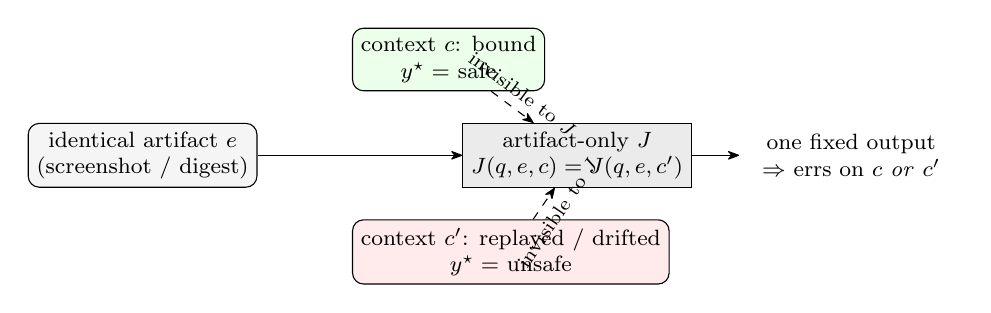
\begin{tikzpicture}[
  font=\footnotesize,
  node distance=5mm and 8mm,
  art/.style={draw,rounded corners,align=center,inner sep=3pt,fill=black!4,minimum height=6mm},
  ctx/.style={draw,rounded corners,align=center,inner sep=3pt,minimum height=6mm},
  jud/.style={draw,align=center,inner sep=3pt,minimum height=6mm,fill=black!8},
  >={Stealth[round]}]
\node[art] (e) {identical artifact $e$\\(screenshot / digest)};
\node[ctx,above right=4mm and 12mm of e,fill=green!8] (csafe) {context $c$: bound\\$y^\star=$ safe};
\node[ctx,below right=4mm and 12mm of e,fill=red!8] (cunsafe) {context $c'$: replayed / drifted\\$y^\star=$ unsafe};
\node[jud,right=26mm of e] (j) {artifact-only $J$\\$J(q,e,c)=J(q,e,c')$};
\draw[->] (e) -- (j);
\draw[->,dashed] (csafe) -- (j) node[midway,above,sloped]{\scriptsize invisible to $J$};
\draw[->,dashed] (cunsafe) -- (j) node[midway,below,sloped]{\scriptsize invisible to $J$};
\node[align=center,right=6mm of j,text width=26mm] (out) {one fixed output $\Rightarrow$ errs on $c$ \emph{or} $c'$};
\draw[->] (j) -- (out);
\end{tikzpicture}%
}
\caption{The indistinguishable pair behind Theorem~\ref{thm:separation}. The two inputs present the \emph{same} artifact $e$ but opposite ground truths, differing only in context $c$ (task identity, policy version, provenance) that an artifact-only judge cannot observe. Any such $J$ must return one output on both, so it authorizes an unsafe transition on $c'$ or wrongly declines on $c$---a gap no classification accuracy closes. The binding and ex-ante predicates break the pair by making $c$ observable to the guard.}
\label{fig:indist}
\end{figure}

\paragraph{Scope of the theorem, and what it does \emph{not} settle.} The theorem constrains judges that read the artifact alone; it is what motivates supplying $c$ to the decision at all. It deliberately says nothing about a judge that is \emph{given} $c$ by some channel---for example, one that receives the task identifier, version, and digest as text in its prompt. Such a judge is outside the theorem's scope, and we do not claim the theorem forces it to fail. This matters because our primary confirmatory baseline (J1-IM, \S\ref{sec:study}) is exactly such an information-supplied judge. The separation result therefore does not pre-decide the confirmatory comparison; it only rules out closing the gap by classification accuracy on the artifact. Whether making $c$ available \emph{as prompt text to a probabilistic judge} is as safe as making it available \emph{as deterministic enforcement in the guard} is a separate, empirical question, and is precisely what the confirmatory study is built to answer rather than assume.

\section{Verification Contracts}
A Verification Contract is
\begin{equation}
K=\langle I,P,B,V,A,R\rangle,
\end{equation}
where $I$ contains the declared outcome and immutable constraints; $P$ contains proof obligations committed before evidence; $B$ binds evidence to task, policy version, and context; $V$ is a selective verifier; $A$ defines admissible transitions; and $R$ constructs a decision receipt.

We do not claim this tuple is the only possible decomposition, but we do prove it is \emph{non-redundant}: within an explicit defect model (\S4.5, Theorem~\ref{thm:necessity}) removing any single property admits a harmful transition that the full guard blocks, so no property is dispensable. Minimality thus has two layers we keep separate---a model-internal necessity theorem, and the sharper empirical claim that \emph{real} defects instantiate those witnesses, which each ablation in \S\ref{sec:study} is designed to test.

\subsection{Three-Valued Authorization}
Each authorization predicate evaluates in the three-valued domain $\mathbb{T}=\{\top,\bot,?\}$, where $?$ denotes an unresolved (unknown) state. We adopt Kleene's strong three-valued logic \cite{kleene1952metamathematics,fitting1994kleene}, whose conjunction $\land$ has the relevant clauses $\top\land\top=\top$, $\bot\land x=\bot$ for all $x$, and $\top\land{?}={?}$; the same $\bot$-dominant semantics governs unknown values in databases and monitoring, so we reuse it rather than reinvent it. The decisive design choice is that authorization is read through a \emph{truth-biased} guard $\llbracket\cdot\rrbracket_\top$ that maps only $\top$ to \emph{permit} and collapses both $\bot$ and $?$ to \emph{do-not-permit}. Thus unknown is never truthy: it can never, by any composition rule, be promoted to a permit.

\paragraph{Which predicates actually use the third value.} We are explicit that only one of the four predicates is genuinely three-valued in operation. Ex-ante consistency ($P$, comparing the operative criterion version to the committed one), evidence binding ($B$, comparing the artifact digest and task/version identifiers to their committed values), and reconstructability ($R$, checking that the required receipt fields are present) are \emph{deterministic} comparisons over committed metadata: they carry no calibrated score, no confidence interval, and no conformal set, and evaluate to $\top$ or $\bot$ with $?$ reserved for the degenerate case of a genuinely missing input. The abstain value is therefore load-bearing only for selective verification ($V$), the single predicate backed by a probabilistic module. We keep a common three-valued domain because the guard composes all four uniformly and because $?$ must still propagate when a deterministic input is absent, but we do not claim a novel three-valued treatment of the deterministic predicates.

\paragraph{Splitting selective verification into three levels: observation $O$, calibration $C$, verdict $V$.} The term ``selective verification'' conflates three things that should be separated: the \emph{raw observation} derived from evidence, the \emph{calibration} that maps an observation to a comparable score, and the \emph{verdict} that discretizes a calibrated score into $\{\top,\bot,?\}$. We therefore decompose $V$ explicitly into a three-level pipeline $O\to C\to V$. \emph{Observation level $O$}: the judge or forensic module emits a raw signal from evidence (e.g.\ a per-obligation model judgment or risk score). \emph{Calibration level $C$}: the raw signal is mapped to a score $p\in[0,1]$ with a calibration guarantee; we require it to be calibrated \cite{guo2017calibration} and, where a distribution-free coverage guarantee is available, to expose a conformal prediction set at a preregistered risk level $\alpha$ \cite{vovk2005algorithmic,angelopoulos2023conformal}, and the quality of this level is measured \emph{independently} by preregistered calibration diagnostics (ECE and reliability diagrams; see Section~7). \emph{Verdict level $V$}: the predicate value is obtained by a \emph{two-threshold} rule fixed ex ante: $\phi_V=\top$ if the calibrated lower bound exceeds an acceptance threshold, $\phi_V=\bot$ if the calibrated upper bound falls below a rejection threshold, and $\phi_V={?}$ otherwise---i.e.\ whenever the confidence interval straddles the decision boundary, or the conformal set is not a singleton. This decomposition lets us attribute failures of ``wrong observation,'' ``broken calibration,'' and ``mis-set verdict threshold'' to distinct levels rather than lumping them into a single $V$. This is where uncertainty is \emph{preserved rather than rounded}: a score of $0.73$ with a wide interval yields $?$ (abstain), not a forced $\top$. The thresholds and $\alpha$ are frozen before data (Section~\ref{sec:study}). We stress the boundary of what this buys: the discretization guarantees that a \emph{low-margin} or \emph{mis-calibrated} judgment surfaces as $?$ rather than as a rounded $\top$, but it does not prevent a confidently \emph{wrong} $\top$---a judgment that is well inside the acceptance region yet factually incorrect---from passing the guard. That residual risk is not addressed by the semantics and is exactly the quantity the confirmatory risk--coverage evaluation measures against independently rated harm.

A positive action is eligible only when
\begin{align}
\mathrm{Authorize}(K,e,o,h,a^+)={}&\mathrm{Stable}(P)\land\mathrm{Bound}(B,e)\notag\\
&\land\mathrm{Accepted}(V,K,e,o,h)\notag\\
&\land\mathrm{Reconstructable}(R),
\end{align}
and $a^+$ is permitted iff $\llbracket\mathrm{Authorize}(\cdot)\rrbracket_\top=\text{permit}$, i.e.\ iff $\mathrm{Authorize}(\cdot)=\top$ (Figure~\ref{fig:guard}). By the $\bot$-absorbing and $?$-preserving clauses above, a single $\bot$ conjunct rejects and a single $?$ conjunct (absent any $\bot$) abstains; a permit therefore requires \emph{all four} predicates to be independently $\top$. Missing, conflicting, unsupported, or degraded evidence sets the corresponding predicate to $?$, and by truth-bias yields abstention rather than a forced binary.

\begin{figure}[t]
\centering
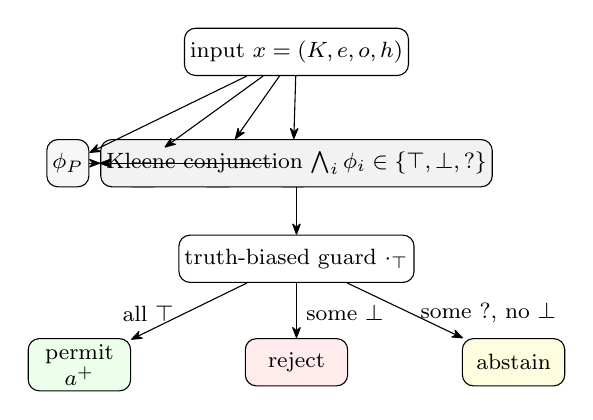
\begin{tikzpicture}[
  font=\footnotesize,
  node distance=6mm and 9mm,
  box/.style={draw,rounded corners,align=center,inner sep=2pt,minimum height=6mm},
  pred/.style={box,fill=black!3},
  outbox/.style={box,minimum width=13mm},
  >={Stealth[round]}]
\node[box] (x) {input $x=(K,e,o,h)$};
\node[pred,below left=8mm and 12mm of x] (p1) {$\phi_P$};
\node[pred,right=4mm of p1] (p2) {$\phi_B$};
\node[pred,right=4mm of p2] (p3) {$\phi_V$};
\node[pred,right=4mm of p3] (p4) {$\phi_R$};
\node[box,below=8mm of x,fill=black!5] (conj) {Kleene conjunction $\textstyle\bigwedge_i\phi_i\in\{\top,\bot,?\}$};
\node[box,below=6mm of conj] (guard) {truth-biased guard $\llbracket\cdot\rrbracket_\top$};
\node[outbox,below left=7mm and 6mm of guard,fill=green!8] (permit) {permit\\$a^+$};
\node[outbox,below=7mm of guard,fill=red!8] (reject) {reject};
\node[outbox,below right=7mm and 6mm of guard,fill=yellow!12] (abst) {abstain};
\draw[->] (x) -- (p1); \draw[->] (x) -- (p2);
\draw[->] (x) -- (p3); \draw[->] (x) -- (p4);
\draw[->] (p1) -- (conj); \draw[->] (p2) -- (conj);
\draw[->] (p3) -- (conj); \draw[->] (p4) -- (conj);
\draw[->] (conj) -- (guard);
\draw[->] (guard) -- node[left,pos=.55]{all $\top$} (permit);
\draw[->] (guard) -- node[right,pos=.55]{some $\bot$} (reject);
\draw[->] (guard) -- node[right,pos=.55]{some $?$, no $\bot$} (abst);
\end{tikzpicture}
\caption{The authorization guard as a decision system. The four property predicates evaluate independently in $\{\top,\bot,?\}$; their Kleene conjunction is read by the truth-biased guard, which permits $a^+$ only on unanimous $\top$, rejects on any $\bot$ (Theorem~\ref{thm:soundness}), and abstains on an unresolved $?$ with no $\bot$. Removing any predicate deletes one incoming edge to the conjunction and thereby its matched harm block (Theorem~\ref{thm:necessity}).}
\label{fig:guard}
\end{figure}

\subsection{Violation-Propagation Invariant}
We isolate the one guarantee the semantics is meant to provide and prove it holds as an interface property, independent of judge quality. We deliberately do \emph{not} name it ``soundness,'' to avoid its being misread as an empirical safety claim; its accurate name is a \emph{violation-propagation invariant}: once a known violation is recorded as $\bot$ by some predicate, it necessarily propagates to the guard's output and blocks the permit. Fix a set $\Phi=\{\phi_1,\dots,\phi_4\}$ of authorization predicates (the four properties) and let each $\phi_i:\mathcal{X}\to\mathbb{T}$ be a partial evaluation over inputs $x=(K,e,o,h)$. Say a positive transition $a^+$ is \emph{unsafely authorized} at $x$ if $a^+$ is permitted while some declared obligation is known-violated at $x$, i.e.\ $\exists i:\phi_i(x)=\bot$.

\begin{theorem}[Violation-propagation invariant]
\label{thm:soundness}
Under the truth-biased three-valued guard, for every input $x$ and every application that gates $a^+$ on $\llbracket\bigwedge_i\phi_i(x)\rrbracket_\top=\text{permit}$, no unsafely authorized transition occurs. Equivalently, a known obligation violation is never masked by unresolved or satisfied co-predicates.
\end{theorem}
\begin{proof}
Suppose $\phi_j(x)=\bot$ for some $j$. By the $\bot$-absorbing clause, $\bigwedge_i\phi_i(x)=\bot$ regardless of the other conjuncts' values in $\{\top,?\}$. The truth-biased guard maps $\bot\mapsto\text{do-not-permit}$, so $a^+$ is not permitted, contradicting the definition of an unsafely authorized transition. Hence none exists.
\end{proof}

The theorem deliberately guarantees \emph{no more} than it can---which is also why we avoid the word ``soundness'': it does not assert that $\phi_i$ evaluates external truth correctly, only that a $\bot$ verdict, once produced, cannot be silently overridden by the composition or by a satisfied sibling. Consequently this invariant is \emph{not} an empirical safety advantage on its own---if a predicate that should read $\bot$ instead reads $\top$ because the underlying observation was wrong, the guard will permit, and the theorem says nothing against it. What the theorem isolates is a compositional failure mode that thresholded scalar judges do exhibit and the guard does not: scalar aggregation lets a high overall score dominate a localized violation, whereas $\bot$-absorption forbids it. Whether the correct $\bot$ is produced in the first place is the probabilistic question the confirmatory study measures, and we are careful not to sell the interface property as if it settled that question.

\begin{proposition}[Abstention monotonicity]
\label{prop:abstain}
Refining an unresolved predicate from $?$ to a definite value can only remove permits, never create a new unsafe one: if $x'\!\succeq x$ resolves some $\phi_i$ from $?$ to $\bot$, the permit set does not grow; if it resolves $?$ to $\top$, any newly created permit still requires all four conjuncts to be $\top$ and hence remains guard-sound by Theorem~\ref{thm:soundness}.
\end{proposition}
\begin{proof}
Resolving $?\to\bot$ makes the conjunction $\bot$ by absorption, revoking any prior permit and adding none. Resolving $?\to\top$ can turn a former $?$-conjunction into $\top$ only if no conjunct is $\bot$; the resulting permit satisfies the antecedent of Theorem~\ref{thm:soundness}, so it is not unsafe. In neither case is an unsafe permit created.
\end{proof}

Proposition~\ref{prop:abstain} is what licenses \emph{selective} deployment: acquiring more evidence (resolving unknowns) is always safe in the guard's sense, so a system may abstain now and safely resume later without a monotonicity violation. This separates our semantics from a two-valued judge, where forcing a decision under an unresolved predicate has no safe default.

\subsection{Contract Properties}
\textbf{Ex-ante consistency} requires decision-relevant obligations to be frozen before the first evidence commitment. Amendments create a new immutable version.

\textbf{Evidence binding} requires accepted artifacts to be committed to task identity, policy version, digest, and required context. A digest establishes identity, not truth. This obligation is the authorization-time analogue of content-provenance standards such as C2PA \cite{c2pa2023spec} and of verifiable credentials \cite{sporny2022vc}, which likewise bind an artifact to an issuer and context; our binding predicate consumes such provenance where available but does not assume it is present or honest.

\textbf{Selective safety} requires unavailable dependencies, hard conflicts, unsupported mandatory inputs, or unresolved uncertainty to abstain. Downstream code may not reinterpret abstention as acceptance.

\textbf{Decision reconstructability} requires an independent auditor to recover the governing policy, evidence commitment, decisive observations, verifier state, and permitted transition.

\paragraph{Enforcement invariant (framing, not a contribution).} If an application enforces $\mathrm{Authorize}=\top$ as a necessary precondition for every $a^+$, an explicitly false contract predicate cannot be silently bypassed by that compliant application. This is a tautological interface property---enforcing a guard means the guard is enforced---stated only to fix terminology. It is not a theorem of external truth, policy legitimacy, or semantic soundness, and we do not list it among our contributions.

\subsection{Relative Non-Redundancy of the Four Properties}
Section~4.1 declined to assert minimality by fiat, and we do \emph{not} claim ``minimality'' in any general sense. We now prove a narrower property inside an explicit defect model---\emph{relative non-redundancy}: relative to the enumerated defect family, no property is redundant, because dropping any one admits a harmful transition that the full guard blocks. The theorem is a statement \emph{about the guard over a modeled defect family}; whether real defects instantiate these witnesses is the separate empirical question our ablations test, and we keep the two claims strictly apart. It does \emph{not} claim the four properties are a minimal sufficient set against every possible defect, only that within the modeled family each one is individually indispensable.

We first name, in Definition~\ref{def:harm}, the harms the guard exists to prevent. Let a \emph{world} $w$ fix, for an input $x=(K,e,o,h)$, the ground facts a downstream consequence depends on: whether the criterion in force at evidence time accepts $e$, whether $e$ is bound to this task and version, whether mandatory observations are validly resolved, and whether the transition is later reconstructable.

\begin{definition}[Authorization and audit harm]
\label{def:harm}
A permitted transition $a^+$ at $(x,w)$ is an \emph{authorization harm} $H_{\mathrm{auth}}$ if $w$ makes $a^+$ transfer value or grant access under a criterion or task binding that does not hold, or wrongfully denies a legitimate submitter. It is an \emph{audit harm} $H_{\mathrm{audit}}$ if $a^+$ is permitted but no auditor can recover the governing policy, evidence commitment, decisive observation, and admitted transition from the receipt alone.
\end{definition}

\begin{definition}[Property-matched defect family]
\label{def:defects}
For each property $i\in\{P,B,V,R\}$ let $D_i$ be the set of inputs exhibiting exactly its matched defect and no other: $D_P$, the operative criterion differs from the committed one (post-hoc drift); $D_B$, $e$ is well-formed but bound to another task or version (replay); $D_V$, a mandatory observation is unavailable, unsupported, or hard-conflicting (forced binary); $D_R$, the receipt omits a field required to reconstruct the decision. Each $\phi_i$ is the predicate that evaluates to $\bot$ on $D_i$ (for $P,B$), to $?$ on $D_V$, and---for $R$---to $\bot$ when reconstructability is not established.
\end{definition}

Write the full guard as $G=\llbracket\bigwedge_{i\in\{P,B,V,R\}}\phi_i\rrbracket_\top$ and the guard with property $i$ removed as $G_{-i}=\llbracket\bigwedge_{j\neq i}\phi_j\rrbracket_\top$.

\begin{theorem}[Relative non-redundancy]
\label{thm:necessity}
For every property $i\in\{P,B,V,R\}$ there is an input $x_i$ on which $G$ does not permit $a^+$ while $G_{-i}$ does, and on which permitting $a^+$ is an $H_{\mathrm{auth}}$ harm for $i\in\{P,B\}$, an unresolved (forced-binary) harm for $i=V$, and an $H_{\mathrm{audit}}$ harm for $i=R$. Hence no property is redundant: each strictly enlarges the set of blocked harmful transitions.
\end{theorem}
\begin{proof}
Fix $i$ and take $x_i\in D_i$ with all other defects absent, so $\phi_j(x_i)=\top$ for $j\neq i$ and, by Definition~\ref{def:defects}, $\phi_i(x_i)\in\{\bot,?\}$. Then $G_{-i}(x_i)=\llbracket\bigwedge_{j\neq i}\top\rrbracket_\top=\text{permit}$, so the reduced guard authorizes $a^+$. For the full guard, $\bigwedge_j\phi_j(x_i)$ has a $\bot$ or $?$ conjunct at position $i$; by the $\bot$-absorbing and $?$-preserving clauses it equals $\bot$ or $?$, and the truth-biased guard maps both to do-not-permit, so $G(x_i)$ does not permit. The permitted transition under $G_{-i}$ is harmful in the stated sense: on $D_P$/$D_B$ the world makes $a^+$ act under a criterion/binding that does not hold ($H_{\mathrm{auth}}$); on $D_V$ it forces a verdict with no valid observational basis; on $D_R$ it commits a transition no auditor can reconstruct ($H_{\mathrm{audit}}$). Thus dropping $i$ admits a harm the full guard blocks, for every $i$.
\end{proof}

Theorem~\ref{thm:necessity} is all of the ``minimality'' intuition we are willing to formalize, properly named \emph{relative non-redundancy}: the four predicates are logically independent guards, each the unique blocker of its matched harm within the model, so none can be deleted without reopening a harmful transition. It does \emph{not} claim the four are jointly sufficient against harms outside $\bigcup_i D_i$, nor that no smaller alternative decomposition exists; that is bounded next.

Table~\ref{tab:defects} lays the family out along the axis that connects this necessity result to the separation theorem: the \emph{discriminating fact} each defect turns on. For $P$ and $B$ that fact is a piece of committed context---the operative criterion version, the task/version the artifact was captured for---that is by construction \emph{absent from the artifact} and therefore invisible to an artifact-only judge (Theorem~\ref{thm:separation}); the guard resolves it by deterministic comparison against the frozen commitment, not by inference. For $V$ the fact is the very \emph{availability} of a mandatory observation, which a binary judge cannot express and must instead fabricate as a forced verdict; the abstain value is what makes it representable. For $R$ the fact is post-hoc: whether the record suffices for reconstruction, which no verdict-time confidence can supply. Reading the table top to bottom, the two $\bot$-valued rows are exactly the cases the separation theorem predicts an artifact-only judge cannot close, the $?$ row is the case a two-valued judge cannot even name, and the $R$ row is orthogonal to the judge entirely---so the four are not an arbitrary list but a partition of the ways an authorization can be wrong that a probabilistic verdict, alone, cannot cover.

\begin{table*}[t]
\centering
\footnotesize
\caption{The property-matched defect family of Definition~\ref{def:defects}, organized by the fact each defect turns on. The last column states why a probabilistic artifact-only judge cannot, in principle, close the case---linking the necessity result (Theorem~\ref{thm:necessity}) to the separation result (Theorem~\ref{thm:separation}).}
\label{tab:defects}
\begin{tabular}{@{}llllc@{}}
\toprule
Property & Defect $D_i$ & Discriminating fact & Guard's resolution & \shortstack{Predicate\\value on $D_i$} \\
\midrule
$P$ (ex-ante criterion) & Post-hoc criterion drift & Operative vs.\ committed criterion version & Equality vs.\ frozen commitment & $\bot$ \\
$B$ (evidence binding) & Cross-task / version replay & Task+version the artifact was bound to & Equality vs.\ committed binding & $\bot$ \\
$V$ (selective verdict) & Forced binary under missing/conflicting obs. & Whether a mandatory observation resolves & Emit $?$; abstain rather than guess & $?$ \\
$R$ (reconstructability) & Receipt omits a decisive field & Whether the record supports later audit & Require complete receipt fields & $\bot$ \\
\bottomrule
\end{tabular}
\end{table*}

\begin{proposition}[Relative completeness over the modeled defects]
\label{prop:completeness}
Suppose every unsafe or unauditable input in the confirmatory scope lies in $\bigcup_{i}D_i$ (each negative carries at least one matched defect). Then $G$ permits no $H_{\mathrm{auth}}$ or $H_{\mathrm{audit}}$ transition: the guard is sound (Theorem~\ref{thm:soundness}) and complete relative to the modeled defect family.
\end{proposition}
\begin{proof}
Let $x$ be unsafe or unauditable. By hypothesis $x\in D_i$ for some $i$, so $\phi_i(x)\in\{\bot,?\}$; by absorption/preservation $\bigwedge_j\phi_j(x)\neq\top$, and the guard does not permit. Conversely any permitted $x$ has $\phi_j(x)=\top$ for all $j$, hence $x\notin\bigcup_iD_i$ and is neither unsafe nor unauditable in scope. Thus permitted $=$ safe-and-auditable within the modeled family.
\end{proof}

We state the assumption of Proposition~\ref{prop:completeness} as a \emph{scope condition}, not a fact about the world: an adaptive adversary can construct harms outside $\bigcup_iD_i$, and the proposition makes no claim there. This is exactly the boundary declared in the threat model and revisited in the limitations, now made precise: completeness is asserted only relative to the enumerated, researcher-instantiated defect families, and the confirmatory study's held-out classes and mutation source test whether that relative guarantee survives distribution shift.

\section{Relation to Adjacent Abstractions}
Software contracts specify conditions over machine-observable state \cite{meyer1997object}; here the postcondition itself must be inferred from incomplete evidence. Proof-carrying code attaches a machine-checkable safety proof \cite{necula1997proof}; open-world screenshots and contextual claims generally admit no such proof. Runtime verification checks traces against formal properties \cite{leucker2009brief}; it does not by itself define evidence sufficiency for an external outcome. Access-control and authorization models---from the classical protection principles of Saltzer and Schroeder \cite{saltzer1975protection} through capability-based composition \cite{miller2006capability} to modern policy-as-code engines \cite{opa2023}---decide permissions over trusted, machine-observable subjects and objects; the open-world setting differs precisely in that the decisive fact (did the outcome occur, under which criterion) is itself uncertain and inferred, so the policy must gate on a probabilistic observation rather than on authenticated state. Selective prediction adds abstention but not ex-ante commitment, task binding, or downstream enforcement. Provenance records lineage, while a complete lineage record need not explain which obligation authorized a transition. Finally, the human-AI reliance literature shows that raw model confidence often miscalibrates human trust and that combined human-AI teams do not reliably beat the better agent alone \cite{schemmer2023reliance,vaccaro2024combinations}; our human study (Section~\ref{sec:study}) is designed around exactly this risk, measuring inappropriate reliance rather than assuming structured evidence helps.

\paragraph{Cryptographic assurance of integrity vs.\ authorization of an outcome.} A security reader will ask why the guard is not simply an instance of three mature integrity mechanisms. Blockchain oracles---from Town Crier's authenticated feeds \cite{zhang2016towncrier} through DECO's TLS-oracle proofs \cite{zhang2020deco} to production oracle networks \cite{ellis2017chainlink} and legacy-compatible decentralized identity \cite{maram2021candid}---and the broader oracle problem \cite{caldarelli2020oracle} authenticate the \emph{source} of an off-chain datum: they prove a value truly originated from a given server or TLS session. Trusted execution environments \cite{costan2016sgx,intel2021tdx,sabt2015tee} attest that a specified \emph{computation} ran unmodified inside an enclave. Zero-knowledge and verifiable-computation systems \cite{goldwasser1989knowledge,parno2013pinocchio,ben2014succinct,thaler2022proofs} prove that a committed input was processed by a fixed function correctly. All three are complementary to, not substitutes for, a Verification Contract, for one structural reason: each certifies the \emph{integrity of a channel or a computation}, whereas the open-world question is the \emph{eligibility of an uncertain outcome}. A TLS-authenticated screenshot, an enclave-attested judge, and a ZK-proved classification are all fully compatible with the four defects of \S3: the artifact can be genuinely fetched, the judge can run untampered, and the proof can be valid, while the criterion silently drifted, the evidence was replayed from another task, a mandatory provider was down, or the receipt is unreconstructable. These mechanisms answer ``was this byte string faithfully obtained and processed?''; they do not answer ``is this outcome, under this frozen criterion and this binding, allowed to move state?'' A fourth adjacent line, settlement finality---the point at which a transfer becomes irreversible under a consensus rule, whether probabilistic \cite{nakamoto2008bitcoin,garay2015backbone} or provably final \cite{buterin2020gasper,buchman2016tendermint}---is likewise orthogonal: it governs \emph{when} a state change can no longer be undone, not \emph{whether} the evidence ever authorized it, and it is precisely because settlement is irreversible that the authorization decision preceding it must be made under a frozen criterion. The guard consumes these mechanisms' outputs as \emph{stronger evidence channels}---an attested $V$, a provenance-authenticated $B$---but its own contribution, anchoring the permit to external downstream harm rather than to channel integrity, is orthogonal to all of them (Table~\ref{tab:positioning}). Their well-documented failure modes---such as transient-execution attacks that break enclave confidentiality \cite{vanbulck2018foreshadow}---are themselves why we treat these as hardenable inputs rather than as the authorization boundary.

No component is claimed as individually novel. The contribution is the authorization boundary joining precommitment, binding, selective decision, and reconstructable transition, together with a property-aligned evaluation whose ground truth is external downstream harm rather than the boundary's own rule.

Table~\ref{tab:positioning} makes the gap concrete along the five dimensions the authorization boundary must cover. Each adjacent line of work addresses a subset---selective prediction contributes abstention, provenance contributes binding, policy-as-code and software contracts contribute ex-ante commitment over \emph{trusted machine state}---but none jointly commits the acceptance rule before evidence, binds an \emph{uncertain} artifact to task and version, abstains under unresolved observation, anchors evaluation to external harm rather than to its own verdict, and emits a reconstructable receipt. The last row is the only fully populated one; that pattern, not the novelty of any single cell, is the contribution.

\begin{table*}[t]
\centering
\footnotesize
\caption{Positioning against adjacent abstractions. $\bullet$: directly provides the property as a design goal; $\circ$: provides it partially or only incidentally (e.g.\ over trusted, machine-observable state, or as a byproduct such as lineage); ---: not addressed. ``Ground truth $=$ external harm'' asks whether the approach's correctness is judged against a consequence \emph{outside} its own decision rule.}
\label{tab:positioning}
\begin{tabular}{@{}lccccc@{}}
\toprule
Approach & \shortstack{Ex-ante rule\\commitment} & \shortstack{Uncertain-artifact\\task/version binding} & \shortstack{Selective\\abstention} & \shortstack{Ground truth $=$\\external harm} & \shortstack{Reconstructable\\receipt} \\
\midrule
LLM-as-a-Judge \cite{zheng2023judging,liu2023geval} & --- & --- & $\circ$ & --- & --- \\
Selective prediction \cite{geifman2017selective,hendrickx2024reject} & --- & --- & $\bullet$ & --- & --- \\
Media forensics \cite{verdoliva2020media} & --- & $\circ$ & --- & --- & --- \\
Content provenance / VC \cite{c2pa2023spec,sporny2022vc} & --- & $\bullet$ & --- & --- & $\circ$ \\
Blockchain oracles / zkTLS \cite{zhang2016towncrier,zhang2020deco} & --- & $\circ$ & --- & --- & $\circ$ \\
Trusted execution env.\ \cite{costan2016sgx,intel2021tdx} & --- & $\circ$ & --- & --- & $\circ$ \\
ZK / verifiable computation \cite{parno2013pinocchio,ben2014succinct} & $\circ$ & $\circ$ & --- & --- & $\circ$ \\
Access control / policy-as-code \cite{saltzer1975protection,opa2023} & $\circ$ & $\circ$ & --- & --- & $\circ$ \\
Software contracts / PCC / RV \cite{meyer1997object,necula1997proof,leucker2009brief} & $\circ$ & --- & --- & --- & $\circ$ \\
\midrule
\textbf{Verification Contract (this work)} & $\bullet$ & $\bullet$ & $\bullet$ & $\bullet$ & $\bullet$ \\
\bottomrule
\end{tabular}
\end{table*}

\paragraph{Positioning.} This work does not improve any model; it specifies and evaluates an authorization protocol wrapping a judge. Its natural home is therefore the intersection of trustworthy-ML evaluation and systems security---venues concerned with policy enforcement, provenance, and auditable settlement---rather than a modeling track. We state this explicitly so the confirmatory claim is judged as a protocol and evaluation contribution, not as a learning result.

\section{Contract-Governed Verification}
The prototype compiles a natural-language request into typed obligations specifying evidence modality, mandatory status, decision method, and failure behavior. A model-assisted compiler is paired with deterministic fallback so provider failure cannot remove the policy boundary.

Submitted evidence is bound to task identifier, policy version, server receipt time, and artifact digest. Observation modules expose deterministic rule checks, limited forensic risk signals, and per-obligation multimodal judgments. Forensic observations can raise risk or request review but cannot independently prove manipulation. Semantic models cannot override deterministic contract failure.

The verifier records provider, model version, threshold, response validity, and degradation state. Required provider failure, unsupported mandatory evidence, or hard conflict yields unknown. The receipt commits to policy, evidence, observations, decision, admissible transition, and a shared immutable decision identifier.

\paragraph{Reconstructability as a two-phase atomic transaction.} If ``write the receipt'' and ``execute $a^+$'' are separable steps, there is a window---the transition has happened but the receipt is not yet persisted, or vice versa---in which the truth of $\phi_R$ is ill-defined. We therefore specify the authorize--execute chain as a \emph{two-phase commit}: in the \emph{prepare} phase the guard evaluates the four predicates against frozen commitments and writes the complete receipt to a durable log, without executing $a^+$; in the \emph{commit} phase, if and only if the receipt is persisted and $\phi_R=\top$, executing $a^+$ and marking the receipt as effective are performed as a single \emph{atomic} operation. Failure in either phase rolls back to ``not authorized,'' never leaving a ``transferred but not reconstructable'' intermediate state. Thus $\phi_R$ is not an after-the-fact check but a \emph{precondition} of the commit phase: a production integration must bind verification, receipt persistence, and settlement atomically; the reference validator is a conformance oracle, not proof that every deployment path enforces the guard. We acknowledge that this only shifts the non-reconstructability risk from application logic onto the correctness of the underlying transactional primitive, and we revisit this residual assumption in the limitations.

\subsection{A Worked Replay Case}
\label{sec:worked}
To make the guard's behavior concrete---and to show it acting on an input a strong judge accepts---we trace one $D_B$ (cross-task replay) bundle end to end. The example is illustrative, drawn from the base-case template family rather than from confirmatory data; no result is claimed from it.

\emph{Setup.} A requester posts task $q_{412}$: ``publish the sentence \texttt{Launch is live} from account \texttt{@acme} before 18:00 UTC.'' At contract creation the obligations are frozen: criterion version $v_3$, required modality \texttt{screenshot}, mandatory provider \texttt{web-archive}, decision method \texttt{selective}, failure behavior \texttt{abstain}. The producer later submits a screenshot $e^\dagger$ that genuinely shows \texttt{Launch is live} on \texttt{@acme}---but the capture was produced for a \emph{different} task $q_{197}$ under criterion version $v_2$, and is being replayed. The presented artifact digest is authentic; only its \emph{binding} is wrong.

\emph{What the judges see.} A generic judge J0 and the policy-aware judge J1, reading the artifact, both report $\mathrm{success}$ at high confidence: the sentence, the handle, and the layout are exactly what the request names. The information-matched judge J1-IM additionally receives, as prompt text, the committed identifiers ($q_{412}$, $v_3$) and the digest recorded at capture ($q_{197}$, $v_2$), and \emph{could} in principle notice that the two task identifiers differ; whether it does depends on the model attending to two identifiers buried in context rather than to the visually convincing screenshot. This is exactly the indistinguishable pair of Figure~\ref{fig:indist}: identical artifact, opposite ground truth, the discriminating fact living only in the context $c$.

\emph{What the contract does.} The guard evaluates the four predicates independently over committed metadata:
\begin{itemize}
\item $\phi_P=\top$: the operative criterion is $v_3$, matching the committed version---no drift.
\item $\phi_B=\bot$: the binding predicate compares the submission's committed task/version $(q_{197},v_2)$ against the contract's $(q_{412},v_3)$ by deterministic equality; they differ, so binding \emph{fails}.
\item $\phi_V=\top$: the selective verifier, reading only the artifact, is confident the sentence is present.
\item $\phi_R=\top$: all receipt fields are present.
\end{itemize}
By $\bot$-absorption, $\bigwedge_i\phi_i=\bot$ regardless of the three satisfied conjuncts, and the truth-biased guard maps $\bot\mapsto$ \emph{reject} (Theorem~\ref{thm:soundness}). The positive action is withheld even though the semantic content is correct and the verifier is confident: the transition is unsafe not because the screenshot is fake, but because it is \emph{not bound to this task}. The receipt records the decisive conjunct ($\phi_B=\bot$, with both digests and both identifier pairs), so an auditor can later reconstruct exactly why authorization was refused---the property J0/J1 cannot supply because they never represented the binding at all.

This single case exhibits every moving part of the paper at once: the separation (identical artifact, context-dependent truth), the load-bearing distinction between an information-supplied judge and a deterministic comparison, $\bot$-absorption overriding a confident $\top$, and reconstructability turning the refusal into an auditable record.

\subsection{A Deployed Settlement Loop as a Reference Instantiation}
\label{sec:instantiation}
The worked example above is described abstractly. To show that a Verification Contract is not a paper construct, we map the six-tuple $K=\langle I,P,B,V,A,R\rangle$ onto the real components of an \emph{independently deployed, continuously operating} settlement loop. That loop realizes a full production cycle: \emph{campaign publication $\to$ evidence binding $\to$ selective verification $\to$ on-chain settlement $\to$ receipt}. To comply with double-blind review, this section deliberately describes the system's capabilities in a \emph{de-identified} manner and does \emph{not} name the platform, its domain, or any contract address; the system's identity, acknowledgements, and on-chain artifact pointers are deferred to the camera-ready version.\footnote{To preserve double-blind review, the name, operator, and on-chain contract addresses of the deployed system described here are withheld during review. A supplement containing the system identity, public contract addresses, and a read-only audit entry point will be provided after acceptance; its content hash is time-stamped together with the preregistration to establish that the system described here existed and ran before submission rather than being constructed after the fact.}

\begin{table}[t]
\centering
\footnotesize
\caption{Field-by-field mapping of the Verification Contract six-tuple $K=\langle I,P,B,V,A,R\rangle$ onto the real components of a deployed settlement loop. The system is described in de-identified form; the last column states when each field is frozen or enforced, to be read against the guard of Figure~\ref{fig:guard} and the two-phase commit of \S\ref{sec:study}.}
\label{tab:instantiation}
\resizebox{\columnwidth}{!}{%
\begin{tabular}{@{}p{2.4cm}p{4.9cm}p{2.9cm}@{}}
\toprule
Contract field & Component in the deployed loop & Frozen / enforced when \\
\midrule
$I$ declared outcome and immutable constraints & Outcome declaration and immutable parameters (reward, deadline, permitted downstream actions) locked at campaign publication & Written at publication; immutable thereafter \\
$P$ ex-ante proof obligations & Acceptance-criteria version and per-obligation checklist frozen at publication & \emph{Before} the first evidence submission \\
$B$ evidence binding & Binding of submitted evidence to campaign id, criteria version, server-side receipt time, and evidence digest & At the moment of evidence submission \\
$V$ selective verifier & Multimodal judgment $+$ deterministic rule/digest checks yielding $\top/\bot/?$; service failure or a hard conflict yields $?$ & At verification time \\
$A$ admissible transitions & Whitelisted on-chain settlement / access-grant actions & Commit phase (two-phase commit) \\
$R$ decision receipt & Immutable receipt with a shared decision identifier emitted per decision (on-chain queryable) & Bound \emph{atomically} to settlement \\
\bottomrule
\end{tabular}%
}
\end{table}

Table~\ref{tab:instantiation} shows the mapping is not a metaphor: the system freezes $I$ and $P$ at campaign publication (ex-ante consistency), computes the binding digest for $B$ at the instant of evidence submission, resolves $V$ through a selective verifier before settling, restricts $A$ to a whitelisted action set, and binds $R$ \emph{atomically} to on-chain settlement---exactly the two-phase commit specified in \S\ref{sec:study}. The abstract authorization boundary of this paper therefore has a counterpart that already runs on a real, irreversible settlement path rather than existing only on paper.

\paragraph{Why these mechanisms can only come from a real system.} The de-identified description above is credible because its load-bearing properties are not ones a paper contract can retrofit; they can only arise from the engineering trade-offs a running system is \emph{forced} into once it must face \emph{irreversible settlement}. First, the binding digest $B$ is computed \emph{server-side} at the instant the evidence is received, time-stamped by an authoritative server clock rather than by the submitter's self-report, so the judgment ``this evidence belongs to this campaign and this frozen criterion'' is tamper-evident and independently recomputable by a third party rather than trusting a client's word. Second, because on-chain settlement is irrevocable, the system interposes a guard \emph{before} the commit (Figure~\ref{fig:guard}): only $V=\top$ proceeds to settlement, $V=?$ (service failure or hard conflict) \emph{never} auto-releases funds but suspends, escrows, or escalates to a human, and $V=\bot$ refuses payment outright---precisely the enforced form, on a real money path, of the two-phase commit of \S\ref{sec:study}. Third, the admissible-transition set $A$ is \emph{physically} narrowed to a whitelist of actions, so the ``blast radius'' of any single wrong decision is bounded by the settlement layer itself rather than relying on the judge's self-restraint. Fourth, the receipt $R$ emitted per decision shares one decision identifier with, and is bound \emph{atomically} to, its on-chain settlement, so reconstructability is not a promise but an already-existing, read-only, anyone-queryable on-chain artifact. It is exactly these constraints---enforced \emph{before} an irreversible action and independently replayable \emph{after}---that constitute evidence a paper contract cannot fabricate and only a deployed system would possess.

\paragraph{As a source of confirmatory data.} Confirmatory data for Group B (external outcomes) is to be \emph{collected from this independently operating production settlement system}: real campaigns produce real evidence submissions, real settlements, and---under dispute---real appeal consequences, whose outcomes are labeled by \emph{raters blind to the contract mechanism}. This is consistent with the independence argument of \S\ref{sec:study} and \S\ref{sec:limitations}: because the system runs independently of our labeling pipeline and the raters are unaware of the protocol internals, external-outcome labels do not collapse into the protocol's own rules. It also partly closes the gap conceded in \S\ref{sec:limitations}---in a production loop the harm on which $V$ turns is an \emph{observed} real settlement/appeal consequence rather than a counterfactual reconstruction. We do not hide the potential conflict of interest: because the deployed system is affiliated with the authors, it is precisely by hiding the system identity, predictions, and settlement state from raters (the blinding protocol of \S\ref{sec:limitations}) that we break the ``using our own system to prove our own system'' loop, and we disclose the relationship in full at camera-ready for readers to judge independently. We reiterate the caveat of \S\ref{sec:limitations}: for the deterministic defect classes ($D_P,D_B$) the anchor still shares inputs with the rules, so real settlement consequences supply a genuinely independent harm signal only for the $V$-dominated classes. During review the main text states only that ``confirmatory data is collected from an independently operating production settlement system and labeled by blinded raters''; the system's identity and on-chain artifacts are supplied at camera-ready.

\section{JOVE-Core}
JOVE-Core covers six digital task classes: social content, account configuration, content publication, form or document submission, time-sensitive digital state, and cross-evidence consistency. Physical execution is outside the confirmatory scope.

The independent unit is a consented base case containing a low-risk request, frozen contract, valid evidence, provenance, and release boundary. Matched variants alter one target property while preserving irrelevant surface features: post-hoc criterion drift, cross-task or cross-version replay, provider failure, integrity conflict, or incomplete receipt. All variants from one base case remain in one split, and no base case contributes to both the calibration and the confirmatory partition.

\paragraph{Ground truth, and the honest limit of its independence.} To avoid defining success as ``agreement with the contract''---which would let a contract-executing system win by construction---the confirmatory label is a \emph{downstream harm} whose \emph{implementation} (which system decided, and how) is hidden from the rater. For each transition we ask whether releasing the positive action would (a) transfer value or grant access on evidence that does not belong to this task or this frozen criterion, or (b) wrongfully deny a legitimate submitter. Raters judge this from the request, the evidence, and the operative criterion, blind to system identity, prediction, mutation category, settlement status, protocol internals, and each other's ratings.

We are candid about what this blinding does and does not achieve. In the researcher-constructed, consented, low-stakes base cases there is no real payment, no real access grant, and no real rejected submitter; the harm is therefore a \emph{counterfactual} judgment about consequences that did not occur. For the deterministic-defect classes ($D_P$ drift, $D_B$ replay) a rater deciding ``does this evidence belong to this task and this frozen criterion'' is, in information terms, re-executing the ex-ante and binding predicates by hand. So for exactly those classes the harm label is blind to the protocol's \emph{implementation} but not informationally orthogonal to the protocol's \emph{rule}: the anchor and the predicate share their inputs, and no labeling protocol can separate them without a real downstream consequence to observe. We therefore do not claim the ground truth is rule-independent in general. Its independence is genuine only for the probabilistic predicate ($V$), where the harm turns on a factual matter (did the claimed outcome actually occur) that the rater assesses without executing the contract, and for classes where a real settlement or contestation consequence is instrumented. For $P$ and $B$ we report results under the explicit caveat that the anchor is a human recomputation of the same rule, and we treat closing this gap---by introducing real settlement and appeal consequences so harm is observed rather than reconstructed---as required future work, not as something the current design achieves. The contract's ``sufficiency under frozen obligations'' remains a \emph{predictor} validated against harm rather than the definition of the target, and a contract that satisfies its own obligations while still producing harm counts against it.

\paragraph{Sample size and adjudication (majority-vote admission, agreement stratification).} The confirmatory set targets 200 base cases yielding at least 600 matched bundles, sized by the power analysis in Section~7.5 to detect the preregistered minimum effect at 80\% power. Each bundle is independently labeled by 3 raters and the harm label is assigned by \emph{majority}. Using ``unanimous agreement of all three raters'' as the admission criterion would systematically \emph{discard the harder-to-adjudicate bundles}, which are likely to be non-randomly enriched in certain defect classes, introducing selection bias into the formal results. We therefore \emph{abandon} unanimity as the admission rule for the main analysis. The main analysis runs on \emph{all} bundles that obtain a majority label---i.e.\ the admission criterion is ``a majority exists''---and $2$--$1$ split bundles are \emph{included} under their majority label rather than held out. To avoid losing agreement information, we \emph{stratify} each bundle by rater agreement (unanimous vs.\ $2$--$1$) and, alongside the main analysis, preregister two agreement sensitivity analyses: (a) re-estimating the primary effect on unanimous bundles only, and (b) weighting $2$--$1$ bundle labels by their uncertainty. If the main analysis (majority-vote admission) and the sensitivity analysis (unanimous admission) disagree in the direction of the effect, we report the discrepancy faithfully rather than presenting whichever is more favorable. Separately, and only as a corpus-level reliability report, we compute Krippendorff's $\alpha$ over the entire labeled set \cite{hayes2007answering} and preregister $\alpha\geq 0.67$ as the acceptance bar for the corpus as a whole; $\alpha$ is never used to admit or exclude individual bundles. Because rater agreement can itself correlate with defect class (Section~\ref{sec:study}), we report admission rates, agreement rates, and the confirmatory effect \emph{per defect class}, so that classes which are harder to adjudicate cannot be silently removed from the classes on which the formal results bear. Irreducible criterion ambiguity is recorded as a labeled category with its prevalence reported, not silently excluded, so exclusion cannot inflate the effect.

\section{Experimental Design}
\label{sec:study}
\subsection{Systems}
J0 is a generic post-hoc judge. J1 is a strong policy-aware judge. J1$+$abstain augments J1 with a confidence-thresholded abstention interface so that coverage can be varied and matched against the contract. J1-IM is the information-matched judge: it receives the identical \emph{input fields} as K-Full's verifier but not the deterministic comparison verdicts over them (see the per-field construction below). J1-DT is the \emph{deterministic tool-augmented} judge: on top of all of J1-IM's fields it is \emph{additionally} granted the ability to call a set of deterministic tools---an identifier/version equality checker and a digest equality checker---and is explicitly prompted that it may invoke them before deciding. K-P, K-B, and K-S add ex-ante policy, binding, and selectivity incrementally. K-Full implements all four properties. Calls, tokens, latency, and monetary cost are reported for every system.

\paragraph{Why J1-DT is needed, and what it tests.} J1-IM alone invites a fairness rebuttal: it must \emph{notice} a mismatch through a probabilistic model's token-level attention to two strings in context, whereas K-Full \emph{enforces} it through a deterministic equality operator; if K-Full wins, a skeptic can attribute it to ``K-Full has a tool and the baseline does not'' rather than to structural enforcement itself. J1-DT closes this escape: it \emph{possesses} the same deterministic checking capability as K-Full, differing only in that these checks are \emph{optional and invoked at the model's discretion} rather than \emph{unconditionally enforced and absorbed as $\bot$} by the guard. Thus K-Full versus J1-IM measures the value of \emph{providing} a deterministic comparison, while K-Full versus J1-DT measures the \emph{incremental} value of making that comparison a mandatory structure rather than leaving it to model discretion---which is precisely the part this paper actually claims. If J1-DT reliably calls the tools on its own and attains K-Full's structural consistency, the paper's ``enforcement beats discretion'' claim is weakened, and we report this faithfully (Section~\ref{sec:results}, condition~(2$'$)).

\paragraph{Per-field construction of J1-IM, and the exact sense of ``information-matched.''} Because ``information versus structure'' is the line this paper contests, J1-IM's input is specified field by field and frozen before data. J1-IM receives, in its prompt, every \emph{input} that K-Full's verifier consumes---the raw evidence, the frozen criterion text, the declared obligations, the committed task and version identifiers, the committed and the presented artifact digests, and the provider degradation state---rendered as text. It does \emph{not} receive the \emph{outcome} of any comparison: whether the presented digest equals the committed one, whether the version matches, the abstention decision, or the receipt. Those outcomes are the structural enforcement under test.

We are precise about what is and is not matched here, because it is the crux of the whole design. J1-IM is matched on the raw information available to the decision: it is handed exactly the same fields, including both digests and both version identifiers, and could in principle report a mismatch. It is \emph{not} handed the deterministic equality verdict over those fields---that is what K-Full contributes. This is the intended and only fair reading of ``information-matched'': identical inputs, and the difference is solely whether a mismatch is caught by a reliable deterministic comparison or must be noticed by a probabilistic model reading two strings in its context. We do not claim a text LLM will recompute a hash; the point is the opposite---binding is valuable precisely because the equality check is delegated to a deterministic operator rather than left to a model's token-level reading, and the confirmatory contrast measures how much that delegation is worth. Handing J1-IM the comparison verdict itself would make it K-Full, so we do not; withholding the input fields would make it artifact-only and trivially lose by Theorem~\ref{thm:separation}, so we do not do that either. The baseline sits deliberately between those two, and every field in its prompt is logged in the preregistered field map so it cannot be silently strengthened or weakened.

\subsection{Primary Endpoints: Separating Structural Consistency from External Outcome}
Compressing the effect of all four properties into a single ``unsafe positive transition rate'' conflates two epistemically different claims: first, whether the guard \emph{structurally} enforces the deterministic obligations it promises ($P$ ex-ante consistency, $B$ binding, $R$ reconstructability); and second, whether the guard actually reduces an \emph{external, independently rated} downstream harm whose discriminating fact is probabilistic (chiefly via $V$). The truth of the former can be fixed unambiguously by deterministic recomputation; the latter depends on blinded harm labels. We therefore \emph{split} the confirmatory endpoint into two groups, preregistered separately.

\paragraph{Endpoint group A (structural consistency, deterministic).} For each deterministic predicate $i\in\{P,B,R\}$ the endpoint is the \emph{structural-violation escape rate}---the fraction of bundles carrying a matched defect $D_i$ that are erroneously permitted $a^+$. Its truth is given by deterministic recomputation against frozen commitments, with no rater involved, so it is an alignment check on \emph{whether the mechanism operates as defined}, not an external-validity claim. We expect K-Full to attain 0 on these endpoints by construction (the empirical mirror of Theorem~\ref{thm:necessity}) and present it as a \emph{falsifiable implementation-correctness check}: any nonzero value exposes an implementation defect rather than validating the abstraction's value.

\paragraph{Endpoint group B (external outcome, independently rated).} The primary \emph{scientific} endpoint is the unsafe positive transition rate---an independently rated downstream harm, defined in Section~7---evaluated as a \emph{paired comparison} at coverage levels matched across systems. The discriminating fact for this endpoint lies chiefly in the cases handled by the probabilistic predicate $V$, and its truth is given by raters blind to the protocol implementation, so it carries the paper's external-validity claim. The primary contrast is K-Full versus J1-IM, because it holds the input information fixed and varies only whether enforcement is structural: it is the contrast that most directly isolates the paper's thesis. It is not, however, the sole route to falsification; the full set of preregistered falsification conditions is enumerated in Section~\ref{sec:results} and any one of them refutes the central claim. K-Full versus J1$+$abstain is a secondary comparison reported over the risk--coverage curve where that curve is well defined (see the caveat below); the earlier fixed ``$\geq 70\%$'' point is retained only as one labeled slice of a sensitivity analysis, since J1 has no native coverage control and forcing one is itself a design choice.

We insist on separating groups A and B because adding them would let a guard that is \emph{structurally} correct but useless on \emph{external outcomes} inflate its total score via deterministic zeros on $P/B/R$. Only group B may be used to claim empirical superiority of Verification Contracts over information-alignment baselines.

\paragraph{Caveat on curve-based comparison.} K-Full and J1$+$abstain do not share a common coverage mechanism: J1$+$abstain traces a smooth curve as its confidence threshold sweeps, whereas K-Full's deterministic predicates ($P,B,R$) are hard gates that do not vary with a coverage knob, so its selective behavior varies only through the probabilistic predicate $V$. We therefore treat the two objects as \emph{not} lying on a common coverage axis and do \emph{not} report a single paired AURC difference between them as if it were well defined. Instead we compare K-Full against J1$+$abstain only at explicitly matched acceptance-coverage points, restricted to the defect classes on which $V$ (and hence a coverage sweep) is the operative predicate; AURC is reported per system as a within-system summary, not as a cross-system paired area difference.

\paragraph{Harm is not a scalar: $H_{\mathrm{FA}}$, $H_{\mathrm{FR}}$, $H_{\mathrm{AUDIT}}$.} Treating ``harm'' as a single scalar conflates errors that point in opposite directions. We therefore decompose the outcome harm explicitly into three \emph{independent} components, each reported separately and never summed a priori: (a) \emph{false-accept harm} $H_{\mathrm{FA}}$---permitting an unsafe positive transition that should have been blocked (i.e.\ the unsafe positive transition rate, the paper's primary scientific endpoint); (b) \emph{false-reject harm} $H_{\mathrm{FR}}$---blocking or abstaining on a safe transition that should have been permitted, at the cost of availability and throughput; and (c) \emph{audit harm} $H_{\mathrm{AUDIT}}$---the receipt failing to support after-the-fact reconstruction even when the transition decision is correct (missing decisive obligation, evidence commitment, or degraded path). The three are measured on different loss scales, serve different stakeholders, and summing them would mask a degenerate solution that lowers $H_{\mathrm{FA}}$ by manufacturing large $H_{\mathrm{FR}}$. We form a weighted combination only when a loss matrix is explicitly declared, and that matrix is swept as a sensitivity dimension (below).

\paragraph{Operationalizing calibration.} Rather than invoke ``calibration'' loosely, we preregister its measurement and thresholds: the $C$-level scores are assessed by expected calibration error (ECE, 15 equal-frequency bins) \cite{guo2017calibration} and reliability diagrams, and we report the Brier score decomposed into reliability/resolution/uncertainty; when conformal sets are used, we report their empirical coverage at the preregistered $\alpha$ and mean set size \cite{vovk2005algorithmic,angelopoulos2023conformal}. Calibration diagnostics are estimated on the \emph{calibration} partition and verified on the \emph{confirmatory} partition, the two isolated by the leakage gate; calibration quality is reported as an \emph{independent} endpoint and never folded into the unsafe transition rate.

We report, per system, the area under the risk--coverage curve (AURC) as a within-system summary and, at coverage levels matched across systems, the paired risk difference, risk ratio, and 95\% base-case clustered bootstrap intervals with 10{,}000 resamples \cite{efron1994bootstrap}. To stay consistent with the stratified power accounting of Section~7.5 and the per-defect-class admission reporting, the bootstrap resamples \emph{stratified by defect class} and \emph{clustered at the base-case level}, so intervals reflect both class composition and within-base-case correlation rather than treating all bundles as i.i.d. Crucially, the headline effect is reported as a \emph{per-defect-class conditional rate} $P(\text{harm}\mid\text{defect class})$, because the aggregate unsafe rate is a function of author-chosen defect prevalence and is not an interpretable effect size. We additionally report total automation coverage, acceptance coverage, and unsafe acceptance per negative case so a gain cannot be manufactured by collapsing coverage. The confirmatory decision uses a \emph{symmetric} 1:1 false-accept:false-reject loss as the primary operating point, so that no system is favored by a cost asymmetry that happens to reward its preferred error direction; a system that reduces unsafe transitions only by rejecting or abstaining more must still show a net gain under equal costs. Asymmetric losses of 2:1, 5:1, and 10:1---under which a wrongful value transfer or access grant is treated as progressively more costly than a recoverable wrongful rejection---are reported as sensitivity analyses, and we report whether the system ranking is stable across the ratios or reverses at any of them.

\subsection{Mechanism and Generalization}
Property ablations measure criterion-drift transitions, replay acceptance, forced transitions under declared abstention conditions, and audit reconstruction. At least two task classes and one mutation-construction source are held out. A gain that disappears under J1-IM, or that holds only on seen templates or the seen mutation source, is not attributed to the contract abstraction but to information or memorization.

\subsection{Human Studies}
The review study uses three arms, not two, to separate information organization from contract structure: (i) raw task and evidence; (ii) an information-matched packet that presents the same facts in an organized but non-contractual format; and (iii) the structured contract packet, all omitting the final machine verdict. Attributing any effect to the contract abstraction requires arm (iii) to beat arm (ii), not merely arm (i). The primary human outcome is unsafe acceptance; secondary outcomes include accuracy, time, confidence, workload, and inappropriate reliance. A separate audit study compares canonical receipts with ordinary logs and measures reconstruction of policy, decisive obligation, evidence commitment, degradation path, and transition eligibility.

\subsection{Sample Size and Power}
The confirmatory set targets 200 base cases and at least 600 matched bundles, with 3 raters per bundle. The power figures below are a \emph{planning assumption}, not an achieved guarantee: their inputs (baseline rate, minimum effect, intraclass correlation) are \emph{literature-prior / pre-pilot assumed values} not yet estimated from pilot data, so $n=600$ should be read as a \emph{design target} rather than a claim of ``80\% power achieved.'' Under this planning assumption---baseline unsafe rate 0.30 under J1-IM within a defect class, a preregistered minimum detectable effect of an absolute 0.10 reduction (i.e.\ down to 0.20), and base cases clustered at an intraclass correlation of 0.2---the frozen paired clustered bootstrap (\texttt{scripts/power-paired-cluster.mjs}, seed 20260809, 3000 reps, 3 variants per base, two-sided $\alpha=0.05$) requires \emph{110 base cases (330 bundles) within a single defect class} for a planning power of $0.808$. This point estimate clarifies the earlier vague ``about 80\%'': power is defined \emph{within} a class, not on the pooled 600 bundles, and the target of 600 exceeds the single-class requirement of 330 precisely because of the three planning margins below, not through redundancy. Following the audit we add these previously missing planning elements: (i) \emph{stratification}---power is accounted for per defect class, because both the effect and the admission rate may vary by class; we guarantee the \emph{most critical} preregistered defect class reaches the 110-base scale above and report its within-class detectable effect, while remaining classes' within-class effects are reported as exploratory and do not enter the protected confirmatory claim; (ii) \emph{robustness}---the frozen sensitivity sweep (\texttt{scripts/power-sensitivity.mjs}) over baseline $\in\{0.25,0.30,0.35\}$, effect $\geq 0.10$, and intraclass correlation $\in\{0.1,0.2,0.35\}$ yields a per-class required base count between 70 and 140, so the preregistered total of 200 base cases retains margin over the worst case in that domain ($0.35\!\to\!0.25$, $\rho=0.35$, needing 140 base cases); (iii) \emph{attrition}---we assume roughly 15\% sample loss from consent withdrawal, rater attrition, and criterion ambiguity, and inflate the recruitment target accordingly so the net sample still reaches 600; and (iv) \emph{multiplicity}---because we preregister multiple endpoints (structural group A's $P/B/R$, external group B's primary and secondary contrasts, and the J1-DT contrast (2$'$)), we control the false-discovery rate over the external-outcome family with Benjamini--Hochberg and run the primary contrast (K-Full vs.\ J1-IM) first as a protected main test. The baseline rate and intraclass correlation above are \emph{planning priors} to be replaced, per the preregistered \emph{prior-replacement protocol}, by their \emph{power-unfavorable} 95\% bootstrap bounds estimated from the pilot before the scripts are re-run and frozen; the minimum detectable effect of 0.10 is a \emph{decision-anchored} quantity and is \emph{not} re-estimated from any data (pilot or confirmatory) so as not to peek at the confirmatory test. Pilot estimates may only \emph{hold or raise} the frozen sample size; a pilot pointing to a smaller size does not lower the 200-base / 600-bundle floor. If recruitment yields fewer consented cases, or the pilot estimates deviate materially from these priors, the study reports the \emph{achieved} power and downgrades the confirmatory claim to exploratory rather than relaxing the threshold. The registry entry, the frozen analysis scripts, and their commit hash are timestamped before any confirmatory datum is collected.

\section{Results and Falsification}
\label{sec:results}
This section must be generated from frozen scripts after consented confirmatory data are independently labeled. There are currently no confirmatory results to report.

To validate the analysis wiring, table layout, and metric plumbing ahead of data collection, we run the frozen scripts on a \emph{synthetic rehearsal} corpus and verify that each falsification condition is computable end to end. \textbf{We deliberately do not print any synthetic value from the rehearsal into the body}: Tables~\ref{tab:mainresults} and~\ref{tab:propertyresults} show \emph{structural templates} only, with every cell a \texttt{--} placeholder, so that synthetic numbers (even when labeled ``illustrative'') cannot be mistaken for empirical results by downstream readers, secondary citations, or language models. The rehearsal numbers live only in fixture files (\texttt{results/mock-metrics.json}) fenced off by the synthetic-isolation gate (Section~\ref{sec:results} onward, enforced at the \emph{path level} in Reproducibility); they never enter the confirmatory path and are overwritten by frozen confirmatory metrics before submission.

% JOVE_RESULTS_BLOCK_BEGIN
\begin{table*}[t]
\centering
\caption{Main-result \emph{structure template}. All cells are \texttt{--} placeholders: under this protocol snapshot there are no confirmatory numbers to report, and we deliberately print no synthetic value to preclude any misreading as empirical results. Real values will be filled by frozen scripts after consented data are independently labeled. The added J1-DT row is the deterministic tool-augmented judge baseline. UPT denotes the unsafe positive transition rate (i.e.\ $H_{\mathrm{FA}}$); Coverage is automation coverage; AURC and ECE are within-system summaries.}
\resizebox{\textwidth}{!}{%
\begin{tabular}{lrrrrrr}
\toprule
System & UPT $\downarrow$ & Coverage $\uparrow$ & AURC $\downarrow$ & ECE $\downarrow$ & Cost & Latency \\
\midrule
J0 generic judge      & -- & -- & -- & -- & -- & -- \\
J1 policy-aware       & -- & -- & -- & -- & -- & -- \\
J1-IM info-matched    & -- & -- & -- & -- & -- & -- \\
J1-DT deterministic-tool & -- & -- & -- & -- & -- & -- \\
K-P policy contract   & -- & -- & -- & -- & -- & -- \\
K-B binding binary    & -- & -- & -- & -- & -- & -- \\
K-S selective         & -- & -- & -- & -- & -- & -- \\
K-Full                & -- & -- & -- & -- & -- & -- \\
\bottomrule
\end{tabular}%
}
\label{tab:mainresults}
\end{table*}
% JOVE_RESULTS_BLOCK_END

\begin{table}[t]
\centering
\caption{Property-level structure template. All cells are \texttt{--} placeholders; there are no empirical numbers under this protocol snapshot, and real values will be filled by frozen scripts once confirmatory data arrive.}
\resizebox{\columnwidth}{!}{%
\begin{tabular}{lrrr}
\toprule
Property test & Baseline & Contract variant & Paired diff \\
\midrule
Criterion-drift transition & -- & -- & -- \\
Replay acceptance          & -- & -- & -- \\
Forced transition          & -- & -- & -- \\
Audit reconstruction       & -- & -- & -- \\
\bottomrule
\end{tabular}%
}
\label{tab:propertyresults}
\end{table}

The central claim fails under any of the following preregistered conditions; each stands on its own and any one refutes the claim. (1) K-Full does not reduce the per-defect-class unsafe rate relative to J1-IM at matched coverage, with the paired 95\% interval crossing zero. (2) The K-Full advantage over J1-IM vanishes---that is, the effect is explained by information rather than structure. (2$'$) The K-Full advantage over J1-DT (the deterministic tool-augmented judge) vanishes---that is, the effect is explained by \emph{possessing} deterministic checks rather than by making them a \emph{mandatory structure}, refuting the ``enforcement beats discretion'' claim. (3) At matched acceptance coverage on the defect classes where a coverage sweep is well defined (predicate $V$), K-Full does not improve on J1$+$abstain. (4) The gain does not transfer to the held-out task classes or the held-out mutation source; because a deterministic protocol cannot memorize templates, condition~(4) tests generalization of the \emph{learned baselines} and of the effect's attribution, not memorization by K-Full. (5) The reduction in unsafe transitions is accompanied by a drop in acceptance coverage large enough that unsafe acceptance per negative case does not improve---operationalized as no improvement at any matched coverage level, replacing the earlier undefined ``mainly.'' (6) Canonical receipts do not improve independent reconstruction over ordinary logs. If K-P alone accounts for the effect, the later properties are not claimed as necessary. (7) The property ablations are empirical probes of the model-internal necessity result (Theorem~\ref{thm:necessity}), and we state their scope honestly: for the deterministic predicates ($P,B,R$) the theorem's witness restores the matched harm \emph{by construction}, so their ablation confirms the wiring rather than furnishing an independent test, and we do not present it as one. The ablation that carries empirical weight is the probabilistic predicate $V$, where whether removing it reopens the matched harm on real data is genuinely uncertain; if that harm fails to appear, $V$'s necessity does not transfer beyond the defect model and we report it as such rather than claiming empirical minimality. If arm (iii) of the human study does not beat arm (ii), the human benefit is attributed to organization rather than to the contract. If structured human review increases automation bias, that negative result remains in the paper.

\section{Anticipated Objections}
\label{sec:objections}
We state the four objections a critical reader raises first, and answer each against the paper's own claims rather than a weaker paraphrase.

\paragraph{``Isn't this just metadata validation with extra vocabulary?''} If the four predicates were only field checks, the paper would be a naming exercise. The load-bearing content is not that we check task identifiers, but \emph{where the correctness of doing so is anchored}. Separation (Theorem~\ref{thm:separation}) shows an artifact-only judge with unbounded capacity cannot close an indistinguishable pair; necessity (Theorem~\ref{thm:necessity}) shows each dropped predicate reinstates a specific matched harm; the evaluation then anchors ground truth to \emph{external downstream harm}, not to ``did the fields match'' (\S7). A pure metadata validator has none of these: it defines success as its own rule, exactly the tautology our blinded harm label is built to avoid. The claim under test is falsifiable precisely because a metadata validator that satisfies its obligations while still producing harm counts against us (\S\ref{sec:results}, condition 5).

\paragraph{``Why not use a TEE to make the binding unforgeable?''} An enclave can guarantee that the judge \emph{ran unmodified} and that inputs were \emph{received intact}; it cannot decide whether an intact, genuine artifact is \emph{eligible} to authorize this transition under a criterion frozen last week. All four defects of \S3 survive perfect enclave attestation: a replayed screenshot is authentically captured, an attested judge still reads a criterion that drifted, a mandatory provider is still down. A TEE therefore hardens the \emph{evidence channel} feeding $V$ and $B$; it does not supply $P$, selective abstention, or a harm-anchored receipt. We treat enclaves as a strengthening input---and note their own confidentiality failures under transient-execution attacks \cite{vanbulck2018foreshadow} as a further reason not to make attestation \emph{the} authorization boundary.

\paragraph{``Can't a strong LLM just read both hashes and both task IDs and catch the mismatch?''} It can, sometimes---and this is exactly why the information-matched baseline J1-IM \emph{receives both digests and both identifiers verbatim} (\S\ref{sec:study}). We do not claim a language model is incapable of noticing a mismatch; we claim that leaving a binding check to a model's token-level attention over context is unreliable relative to a deterministic equality operator, and the confirmatory K-Full-vs-J1-IM contrast measures the size of that gap on real data. If the gap is zero---if the model reliably catches what the deterministic check catches---condition~(2) of \S\ref{sec:results} fires and the central claim is refuted. The thesis is thus staked on the very experiment this objection proposes.

\paragraph{``With no confirmatory data, why is this a paper and not a proposal?''} Two of the three contributions do not depend on the pending data. The separation and necessity results are theorems, true or false independent of any corpus; the evaluation instrument---preregistered endpoints split into a deterministic structural-consistency group and an independently-rated external-outcome group, a symmetric-loss operating point, per-defect-class conditional rates, the falsification conditions above (including the J1-DT contrast that isolates enforcement from mere tool possession), and the per-field J1-IM construction that makes ``information vs.\ structure'' testable---is itself a contribution, and its adequacy can be judged now. What the data will decide is the empirical magnitude, which we deliberately refuse to preview: the synthetic rehearsal (\S\ref{sec:results}) exists only to prove the pipeline computes each falsification condition, and is fenced off from the confirmatory path by the synthetic-isolation gate.

\section{Limitations and Ethics}
\label{sec:limitations}
A Verification Contract can stabilize an incorrect, discriminatory, or illegitimate policy. Protocol eligibility is not legal, social, or moral legitimacy. Hash binding does not prove capture authenticity. Forensics is incomplete. Models can share correlated errors. Human reviewers can be biased or collude.

Our threat model admits an adaptive, adversarial producer, but the confirmatory data consist of researcher-constructed matched defects. We therefore test robustness only to the attack classes we anticipated and instantiated, not to an adaptive adversary optimizing against the deployed contract. Accordingly, the confirmatory claim is scoped to the six consented digital task classes, low-stakes cooperative settings, and the enumerated defect families; generalization is evaluated only to two held-out classes and one held-out mutation source, and we do not claim generalization to unseen attack strategies or to physical, high-value, or non-cooperative outcomes.

The reconstructability guarantee is specified as a two-phase atomic commit (\S\ref{sec:study}), but this only relocates the non-reconstructability risk rather than eliminating it: it shifts the burden from application logic onto the correctness of the underlying transactional primitive (the durable log and the atomic commit), whose failure modes---partial writes, clock skew across the prepare and commit phases, or a compromised log---are outside what our reference validator certifies. We treat hardening this primitive as a deployment concern and do not claim it is solved here.

The study excludes legal, medical, employment, credit, biometric, intimate, and covert-surveillance decisions. Participation requires explicit consent, bounded retention, minimal evidence burden, and a contestation path. Raw sensitive artifacts remain access-controlled; public artifacts default to commitments, versions, and derived observations.

\section{Reproducibility}
The artifact is organized as a single-direction pipeline that freezes each stage's output as the read-only input to the next, and records a content hash for every stage's output so that any retroactive change upstream is \emph{detectable} (rather than physically impossible): consent registration $\to$ evidence capture $\to$ blinded-packet construction $\to$ independent rating $\to$ system runs and outputs $\to$ scoring $\to$ base-case clustered bootstrap $\to$ paper and figure generation. Each stage is written as schema-validated JSON, raw ratings are append-only, and corrections may only be appended with an adjudication document rather than silently overwriting, so any after-the-fact edit breaks the recorded hash chain and is exposed. We do not claim cryptographic tamper-resistance: an adversary holding full write access can recompute the entire hash chain; what we guarantee is that tampering is \emph{detectable}, not impossible.

A single entry point (\texttt{submission-gate.mjs}) chains six blocking gates and aborts assembly if any fails: (i) \emph{split-leakage}, rejecting any base case whose variants cross the calibration and confirmatory partitions; (ii) \emph{mutation-label leakage}, ensuring mutation classes are hidden from raters and systems; (iii) \emph{privacy}, forcing the public layer to carry only commitments, versions, and derived observations; (iv) \emph{anonymity}, ensuring the blinded packet leaks neither system identity nor raters' scores to one another; (v) \emph{receipt semantics}, verifying that each receipt carries policy, decisive obligations, evidence commitments, a degraded path, and transition eligibility; and (vi) a \emph{synthetic-isolation} gate that enforces \emph{path-level} isolation---rehearsal data written to a separate namespace, synthetic metrics explicitly flagged, and no synthetic- or template-sourced file present on the confirmatory path. Gate (vi) is a mechanical file- and namespace-level check and makes no semantic judgment of content.

Submission requires a consented confirmatory manifest, sealed independent labels, immutable system outputs, real metrics and bootstrap artifacts from the freeze scripts, provenance hashes, regenerated tables and figures, and a clean-environment reproduction. The reproduction bundle is produced by \texttt{build-reproduction-bundle.mjs}, whose \texttt{MANIFEST} sha256 is stable and verifiable and whose \texttt{bundle\_type} field marks it as \emph{method-only} (when confirmatory data is not yet collected) or \emph{results}; \texttt{provenance.json} guarantees that confirmatory rows carry no template or synthetic source. At publication we \emph{plan} to archive the frozen artifact to a public repository with a persistent identifier (DOI) so that deprecated releases remain retrievable and prior results reproducible; under this protocol snapshot that archive has not yet been created. A synthetic rehearsal validates code paths, table layouts, and metric plumbing end to end but \emph{cannot} satisfy any empirical gate: the synthetic-isolation gate fences rehearsal numbers off from the confirmatory path---at the file-path and namespace level---before any confirmatory data is collected.

\section{Conclusion}
Open-world agent reliability cannot end with a model believing that a task succeeded. When probabilistic observations trigger deterministic consequences, a system must state why it is eligible to act. Verification Contracts decompose that eligibility into ex-ante rules, task-bound evidence, selective decision, and reconstructable transition. Whether this abstraction reduces unsafe transitions is an empirical question to be answered by independent, falsifiable evaluation---not by architectural complexity or engineering completeness.

\bibliography{references}
\end{document}
